\documentclass[12pt,a4paper,article,english,firamath]{nsi}
\pagestyle{empty}
\setfontfamily{\brettley}{Cursive standard}[Scale=1.5]
\begin{document}
\titre{Find your figure}
\classe{Euro 1\ere}
\maketitle

\subsection*{Description 1}
{\brettley 

Draw a line segment and a circle passing through its endpoints, whose center is the line segment's midpoint.
Draw two lines passing through the endpoints of the line segment and perpendicular to it. Choose one of the endpoints as the center of a second circle passing through the midpoint of the line segment and draw it.
Draw the line passing through its center and through one intersection of the two circles.}\\[1em]

\begin{tikzpicture}
    \draw[lightgray](0,0)--(\linewidth,0);
\end{tikzpicture}


\subsection*{Figure 4}
\begin{center}
    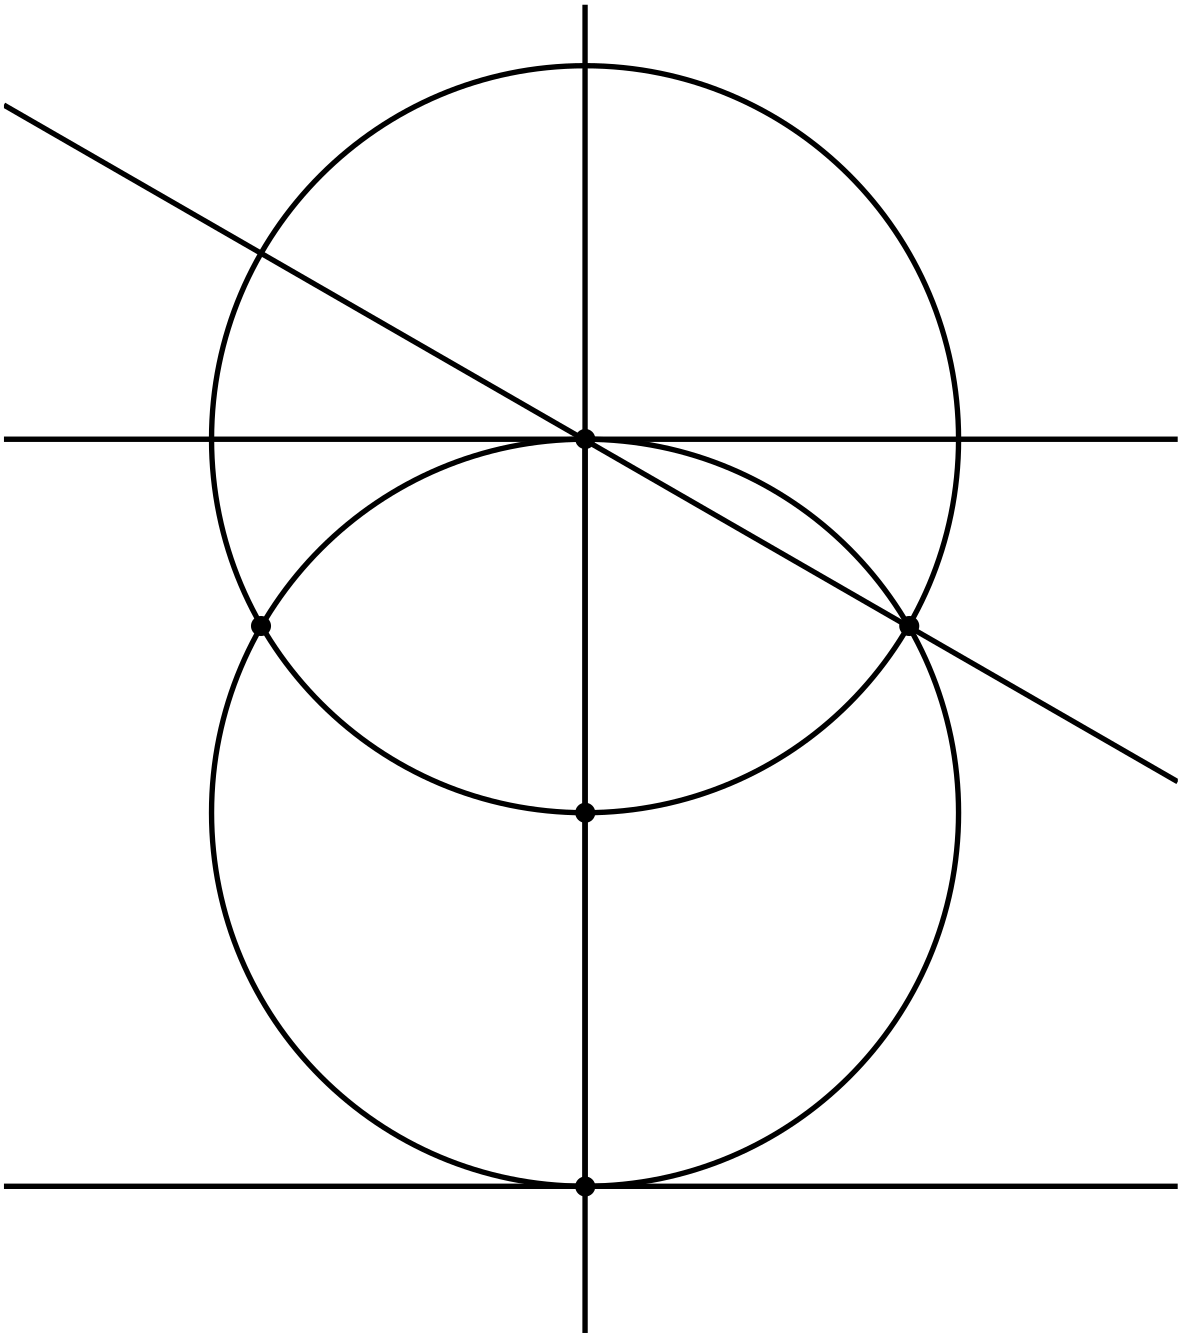
\includegraphics[height=12cm]{img/fig01.png}
\end{center}
\end{document}